\chapter{Design}

I dette kapitel vil vi gennemgå spillet design, og vi vil vise et flow-, klasse- og system sekvensdiagram.

\pagebreak
\section{Flowdiagram}
Indledningsvis tegnede vi et flowdiagram for at skabe overblik over projektet, så vi kunne forstå, hvordan spillet skulle udføres.
Flowdiagrammet blev brugt som baggrund for de efterfølgende diagrammer, som bliver vist i projektet.

\begin{center}
\begin{tikzpicture}[node distance=2cm]
    \node (start) [startstop] {Spillet startes};
    \node (kast) [process, below of=start] {Terningerne kastes};
    \node (passeres) [decision, below of=kast] {Passeres start?};
    \node (ejendom) [decision, below of=passeres, yshift=-1cm] {Er feltet en ejendom?};
    \node (chance) [decision, below of=ejendom, yshift=-1cm] {Er feltet chance?};
    \node (stash) [decision, left of = chance, xshift =-1cm] {Stash \begin{math}
        \geq
    \end{math} ejendomsværdi};
    \node (ejer) [decision, left of = ejendom, xshift = -1cm] {Ejes ejendommen?};
    \node (koeb) [process, left of = ejer, xshift = -2.5cm] {Koeb ejendom};
    \node (betal) [process, left of = passeres, xshift = -2cm] {Betal leje};
    \node (penge) [process, right of = passeres, yshift =-1.9cm, xshift = 0.7cm] {Få penge};
    \node (instrukser) [process, right of = chance, xshift=2.5cm] {Følg instrukser};
    \node (slut) [startstop, left of = stash, xshift =-2.5cm] {Spillet sluttes}; 
    \draw [arrow] (start) -- (kast);
    \draw [arrow] (kast) -- (passeres);
    \draw [arrow] (passeres) -| node[anchor=south] {Ja} (penge);
    \draw [arrow] (passeres) -- node[anchor=west] {Nej}  (ejendom);
    \draw [arrow] (penge) |- (ejendom);
    \draw [arrow] (ejendom) -- node[anchor=south] {Ja} (stash);
    \draw [arrow] (ejendom) -- node[anchor=west] {Nej} (chance);
    \draw [arrow] (chance) -- node[anchor=south] {Ja} (instrukser);
    \draw [arrow] (stash) --node[anchor=west] {Ja} (ejer);
    \draw [arrow] (stash) --node[anchor=south] {Nej} (slut);
    \draw [arrow] (ejer) --node[anchor=south] {Nej} (koeb);
    \draw [arrow] (koeb) |- (kast);
    \draw [arrow] (ejer) -- node[anchor=west] {Ja} (betal);
    \draw [arrow] (betal) |- (kast);
    \draw [arrow] (instrukser) |- (kast);
    \end{tikzpicture}
\end{center}

\section{Klassediagram}

\pagebreak

\section{Systemsekvensdiagram}
Et systemsekvensdiagram viser typisk en form for simplificeret tidslinje over flowet i programmet. Følgende diagram viser interaktionen mellem aktøren spiller og system.

\begin{figure}[H]
    \begin{center}
        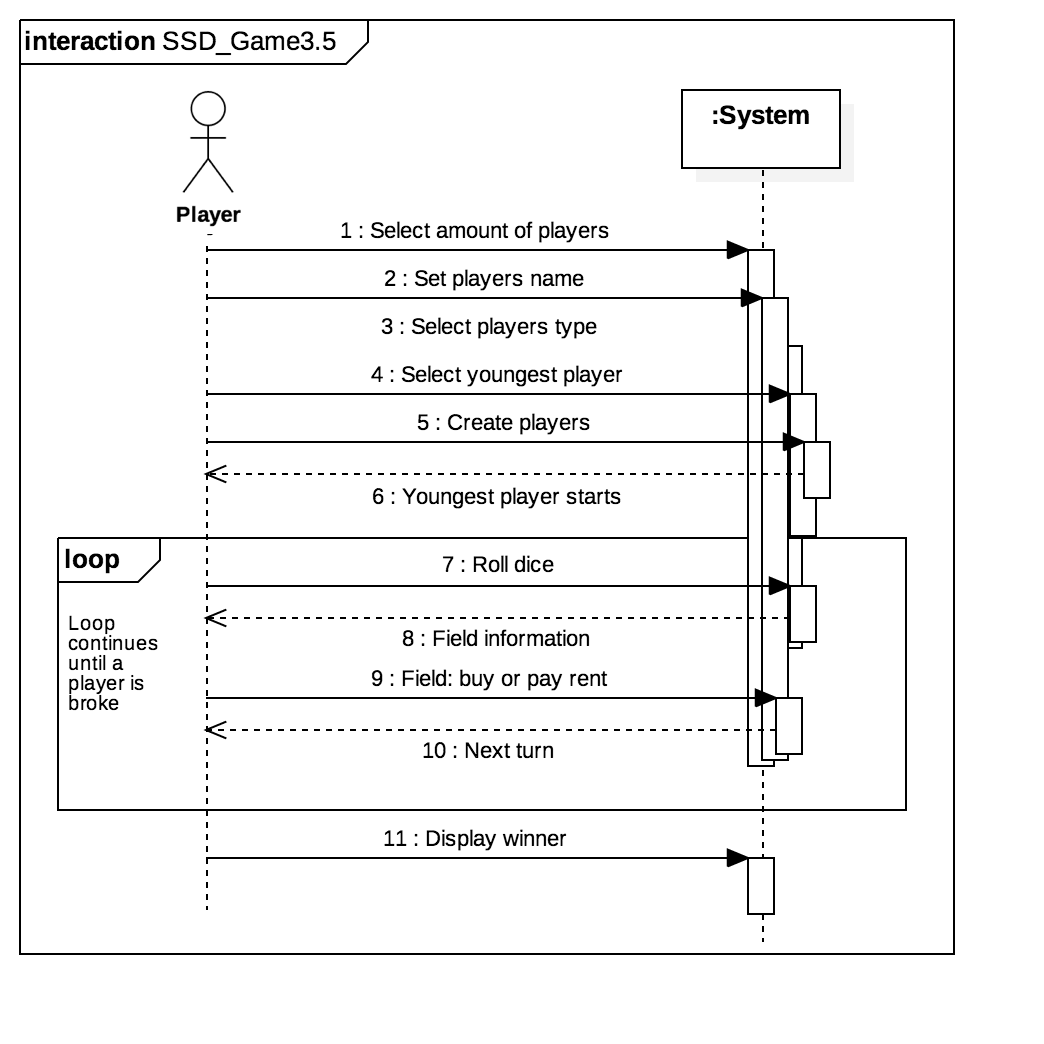
\includegraphics[width=\columnwidth]{graphics/domain/SSD_Game3nw.png}
        \caption{Systemsekvensdiagram}
        \label{fig:systemsekvens_diagram}
    \end{center}
\end{figure}

\noindent Som start bliver der spurgt om antal af spillerer, og da dette udføres visuelt via en dropdown/user selection, udtrykkes denne handling som 'select'.
Eftersom antal af spiller vælges, skal navne på spillerer tastes ind.
Spiller type samt specificering af den yngste spiller gøres på præcis samme måde som i første trin, altså user selection.
Før spillets start tildeles de hver en pengebeholdning afhængig af antallet af spillerer.
På baggrund af trin 6 bliver den yngste spiller den første der starter runden og kaster med terningen.
Roll dice ruller terningen hvor så faceValue afgøre hvilket felt spilleren lander på.
På GUI'en vises feltets oplysninger, samt hvorvidt det er ejet eller ej. Ejes feltet skal der betales leje, ejes det ikke skal det købes.
Efterfølgende er der ekstra tur, vha. 'next turn', hvilket slår igen med terningen, spilleren lander på et felt, og et bestemt scenarie tages i brug, afhængig af felt oplysningerne, hvor så samme procedure følger indtil en spiller ærklæres bankerot.
'Display winner' tæller point på spillerne, og spilleren med den største pengebeholdning vinder spillet, hvilket bliver vist på GUI.\\

\section{Sekvensdiagram}
\begin{figure}[H]
    \begin{center}
        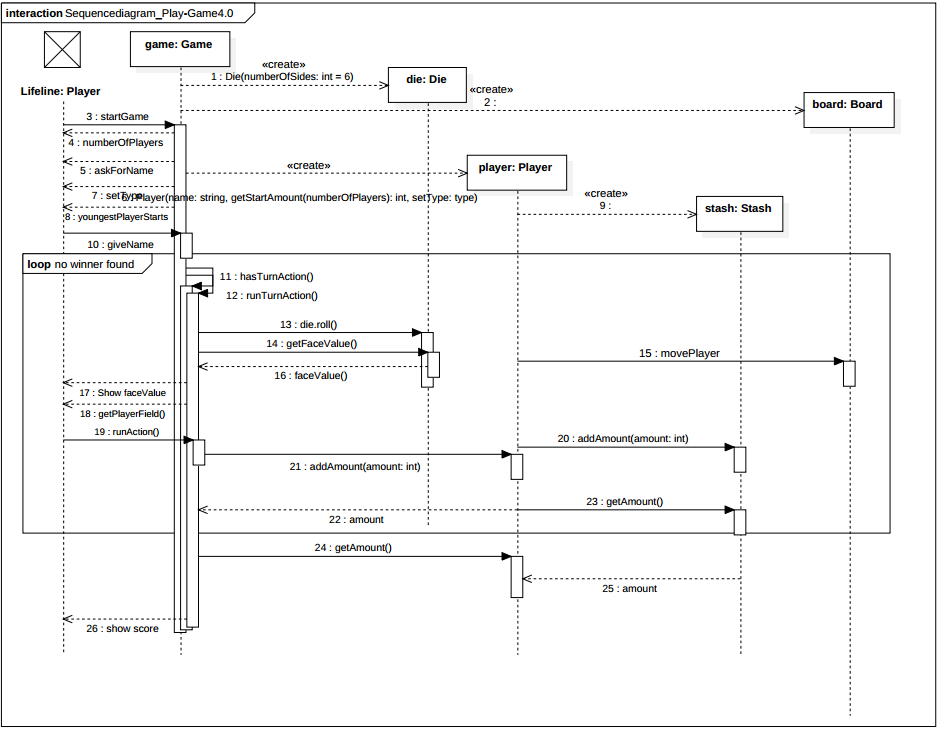
\includegraphics[width=\columnwidth]{graphics/domain/SQdiagram.png}
        \caption{Sekvens diagram}
        \label{fig:sekvens_diagram}
    \end{center}
\end{figure}